%iffalse%\let\negmedspace\undefined
\let\negthickspace\undefined
\documentclass[journal,12pt,onecolumn]{IEEEtran}
\usepackage{cite}
\usepackage{amsmath,amssymb,amsfonts,amsthm}
\usepackage{algorithmic}
\usepackage{graphicx}
\usepackage{textcomp}
\usepackage{xcolor}
\usepackage{caption}
\usepackage{txfonts}
\usepackage{listings}
\usepackage{enumitem}
\usepackage{mathtools}
\usepackage{gensymb}
\usepackage{comment}
\usepackage[breaklinks=true]{hyperref}
\usepackage{tkz-euclide} 
\usepackage{listings}
\usepackage{gvv}                                        
%\def\inputGnumericTable{}                                 
\usepackage[latin1]{inputenc}   
\usepackage{xparse}
\usepackage{color}                                            
\usepackage{array}                                            
\usepackage{longtable}                                       
\usepackage{calc}                                             
\usepackage{multirow}
\usepackage{multicol}
\usepackage{hhline}                                           
\usepackage{ifthen}                                           
\usepackage{lscape}
\usepackage{tabularx}
\usepackage{array}
\usepackage{float}
\newtheorem{theorem}{Theorem}[section]
\newtheorem{problem}{Problem}
\newtheorem{proposition}{Proposition}[section]
\newtheorem{lemma}{Lemma}[section]
\newtheorem{corollary}[theorem]{Corollary}
\newtheorem{example}{Example}[section]
\newtheorem{definition}[problem]{Definition}
\newcommand{\BEQA}{\begin{eqnarray}}
\newcommand{\EEQA}{\end{eqnarray}}
\usepackage{float}
%\newcommand{\define}{\stackrel{\triangle}{=}}
\theoremstyle{remark}
\usepackage{ circuitikz }
%\newtheorem{rem}{Remark}
% Marks the beginning of the document this one
\title{ AE : AEROSPACE ENGINEERING}
\author{EE25BTECH11018-Darisy Sreetej}
\begin{document}
\maketitle

\section{General Aptitude - GA }
\textbf{Q.1-Q.5 carry one mark each.}
\begin{enumerate}
\item The chairman requested the aggrieved shareholders to \dots him.
    \begin{enumerate}
    \begin{multicols}{4}
        \item bare with
        \item bore with
        \item bear with
        \item bare
    \end{multicols}
    \end{enumerate}

\item Identify the correct spelling out of the given options:
    \begin{enumerate}
    \begin{multicols}{4}
        \item Managable
        \item Manageable
        \item Mangeable
        \item Managible
    \end{multicols}
    \end{enumerate}

\item Pick the odd one out in the following:

13, 23, 33, 43, 53

    \begin{enumerate}
    \begin{multicols}{4}
        \item 23
        \item 33
        \item 43
        \item 53
    \end{multicols}
    \end{enumerate}

\item R2D2 is a robot. R2D2 can repair aeroplanes. No other robot can repair aeroplanes.

Which of the following can be logically inferred from the above statements?
    \begin{enumerate}
        \item R2D2 is a robot which can only repair aeroplanes.
        \item R2D2 is the only robot which can repair aeroplanes.
        \item R2D2 is a robot which can repair only aeroplanes.
        \item Only R2D2 is a robot.
    \end{enumerate}

\item If $|9y-6|=3$, then $y^2-\dfrac{4y}{3}$ is \dots.
    \begin{enumerate}
    \begin{multicols}{4}
        \item 0
        \item +1/3
        \item $-1/3$
        \item undefined
    \end{multicols}
    \end{enumerate}

\textbf{Q. 6 - Q. 10 carry two marks each.}

\item The following graph represents the installed capacity for cement production (in tonnes) and the actual production (in tonnes) of nine cement plants of a cement company. Capacity utilization of a plant is defined as ratio of actual production of cement to installed capacity. A plant with installed capacity of at least 200 tonnes is called a large plant and a plant with lesser capacity is called a small plant. The difference between total production of large plants and small plants, in tonnes is \dots.

\begin{figure}[H]
    \centering
    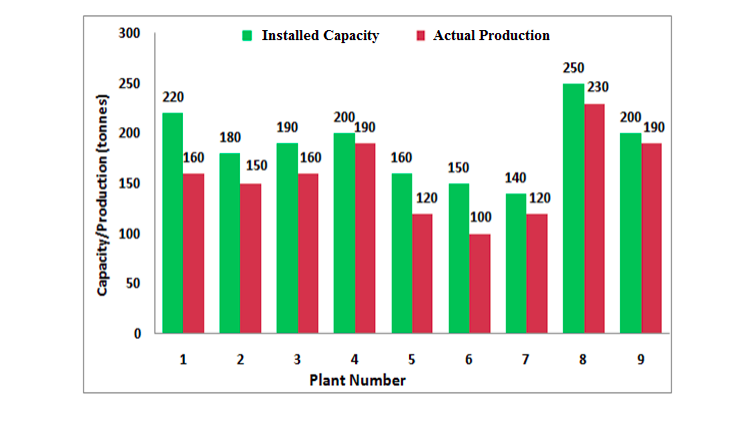
\includegraphics[width=0.5\columnwidth]{figs/Screenshot from 2025-08-16 13-10-40.png}
    \caption{Caption}
    \label{fig:placeholder}
\end{figure}
   
\item A poll of students appearing for masters in engineering indicated that 60\% of the students believed that mechanical engineering is a profession unsuitable for women. A research study on women with masters or higher degrees in mechanical engineering found that 99\% of such women were successful in their professions.
Which of the following can be logically inferred from the above paragraph?
    \begin{enumerate}
        \item Many students have misconceptions regarding various engineering disciplines.
        \item Men with advanced degrees in mechanical engineering believe women are well suited to be mechanical engineers.
        \item Mechanical engineering is a profession well suited for women with masters or higher degrees in mechanical engineering.
        \item The number of women pursuing higher degrees in mechanical engineering is small.
    \end{enumerate}

\item Sourya committee had proposed the establishment of Sourya Institutes of Technology (SITs) in line with Indian Institutes of Technology (IITs) to cater to the technological and industrial needs of a developing country.

Which of the following can be logically inferred from the above sentence?

Based on the proposal,
(i) In the initial years, SIT students will get degrees from IIT.
(ii) SITs will have a distinct national objective.
(iii) SIT like institutions can only be established in consultation with IIT.
(iv) SITs will serve technological needs of a developing country.

\begin{enumerate}
\begin{multicols}{2}
    \item (iii) and (iv) only.
    \item (i) and (iv) only.
    \item (ii) and (iv) only.
    \item (ii) and (iii) only.
\end{multicols}
\end{enumerate}

\item Shaquille O'Neal is a 60\% career free throw shooter, meaning that he successfully makes 60 free throws out of 100 attempts on average. What is the probability that he will successfully make exactly 6 free throws in 10 attempts?

\begin{enumerate}
\begin{multicols}{4}
    \item 0.2508
    \item 0.2816
    \item 0.2934
    \item 0.6000
\end{multicols}
\end{enumerate}

\item The numeral in the units position of $211^{870} + 146^{127} \times 3^{424}$ is \dots
    
\end{enumerate}
\newpage

    \section{Aerospace Engineering - 2016}
\textbf{Q.1-Q.25 carry one mark each.}

\begin{enumerate}
\item  With increase in airfoil thickness, the critical Mach number for an airfoil is likely to  
\begin{enumerate}
 \begin{multicols}{4}
\item  decrease 
\item increase
\item remain unchanged  
\item  be undefined
\end{multicols}
\end{enumerate}
\hfill(GATE AE 2016)



\item Due to a body in potential flow, the velocity at a point A in the flow field is 20 m/s while the free stream velocity is only 10 m/s. The value of coefficient of pressure ($C_p$) at the point A is \dots
\hfill(GATE AE 2016)



\item Which of the following airfoil will have location of the maximum camber at half chord length from the leading edge?  
\begin{enumerate}
    \begin{multicols}{4}
\item NACA 5212
\item NACA 1225 
\item NACA 2215 
\item  NACA 2512
\end{multicols}
\end{enumerate}
\hfill(GATE AE 2016)



\item For a laminar incompressible flow past a flat plate at zero angle of attack, the variation of skin friction drag coefficient ($C_f$) with Reynolds number based on the chord length ($Re_c$) can be expressed as  
\begin{enumerate}
\begin{multicols}{2}
\item  $C_f \propto \sqrt{Re_c}$  
\item  $C_f \propto Re_c$  
\item  $C_f \propto \frac{1}{\sqrt{Re_c}}$  
\item  $C_f \propto \frac{1}{Re_c}$
\end{multicols}
\end{enumerate}
\hfill(GATE AE 2016)



\item Which of the following statement is NOT TRUE across an oblique shock wave?  
\begin{enumerate}
\item Static temperature increases, total temperature remains constant
\item Static pressure increases, static temperature increases
\item  Static temperature increases, total pressure decreases
\item Static pressure increases, total temperature decreases
\end{enumerate}
\hfill(GATE AE 2016)



\item  For a completely subsonic isentropic flow through a convergent nozzle, which of the following statement is TRUE?  
\begin{enumerate}
\item  Pressure at the nozzle exit $>$ back pressure
\item  Pressure at the nozzle exit $<$ back pressure
\item  Pressure at the nozzle exit = back pressure
\item  Pressure at the nozzle exit = total pressure
\end{enumerate}
\hfill(GATE AE 2016)



\item Which of the following aircraft engines has the highest propulsive efficiency at a cruising Mach number of less than 0.5?  
\begin{enumerate}
   \begin{multicols}{2}
\item  Turbofan engine 
\item  Turbojet engine
\item  Turboprop engine
\item  Ramjet engine
 \end{multicols}
\end{enumerate}
\hfill(GATE AE 2016)



\item Air, with a Prandtl number of 0.7, flows over a flat plate at a high Reynolds number. Which of the following statement is TRUE?  
\begin{enumerate}
\item  Thermal boundary layer is thicker than the velocity boundary layer
\item  Thermal boundary layer is thinner than the velocity boundary layer  
\item  Thermal boundary layer is as thick as the velocity boundary layer  
\item  There is no relationship between the thicknesses of thermal and velocity boundary layers
\end{enumerate}
\hfill(GATE AE 2016)



    \item Consider an eigenvalue problem given by $A x = \lambda_i x$.  
    If $\lambda_i$ represent the eigenvalues of the non-singular square matrix $A$, then what will be the eigenvalues of matrix $A^2$?  
    \begin{enumerate}
    \begin{multicols}{2}
        \item $\lambda_i^{4}$
        \item $\lambda_i^{2}$
        \item $\lambda_i^{1/2}$
        \item $\lambda_i^{1/4}$
         \end{multicols}
    \end{enumerate}
    \hfill(GATE AE 2016)



    \item If $A$ and $B$ are both non-singular $n \times n$ matrices, then which of the following statement is NOT TRUE.  
    Note: $\det$ represents the determinant of a matrix.  
    \begin{enumerate}
    \begin{multicols}{2}
        \item $\det(AB) = \det(A) \det(B)$
        \item $\det(A+B) = \det(A) + \det(B)$
        \item $\det(AA^{-1}) = 1$
        \item $\det(A^T) = \det(A)$
        \end{multicols}
    \end{enumerate}
    \hfill(GATE AE 2016)



    \item The total number of material constants that are necessary and sufficient to describe the three-dimensional Hooke's law for an isotropic material is \dots.
\hfill(GATE AE 2016)



    \item Determine the correctness or otherwise of the following statements, [a] and [r]
    \textbf{[a]}: In a plane stress problem, the shear strains along the thickness direction of a body are zero but the normal strain along the thickness is not zero.  
    \textbf{[r]}: In a plane stress problem, Poisson effect induces the normal strain along the thickness direction of the body.  
    \begin{enumerate}
        \item Both [a] and [r] are true and [r] is the correct reason for [a].
        \item Both [a] and [r] are true but [r] is not the correct reason for [a].
        \item Both [a] and [r] are false.
        \item [a] is true but [r] is false.
    \end{enumerate}
    \hfill(GATE AE 2016)



\item Consider four thin-walled beams of different open cross-sections, as shown in the cases below . A shear force of magnitude $F$ acts vertically downward at the location $P$ in all the beams. In which of the following cases, does the shear force induce bending and twisting ?
\begin{figure}[H]
    \centering
    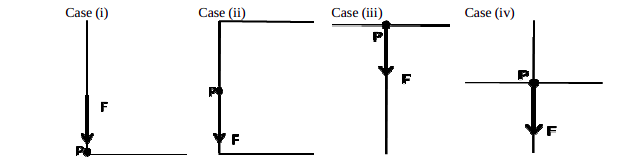
\includegraphics[width=0.5\columnwidth]{figs/Screenshot from 2025-08-15 18-43-29.png}
    \caption{Caption}
    \label{fig:placeholder}
\end{figure}
\begin{enumerate}
\begin{multicols}{4}
    \item \romannumeral 1
     \item \romannumeral 2
      \item \romannumeral 3
       \item \romannumeral 4
       \end{multicols}
\end{enumerate}
\hfill(GATE AE 2016)



\item The effective stiffness of the spring-mass system as shown in the figure below is \dots N/mm.
\begin{figure}[H]
    \centering
    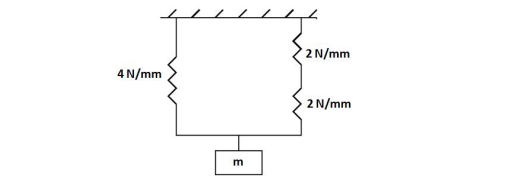
\includegraphics[width=0.5\columnwidth]{figs/Screenshot from 2025-08-15 18-43-56.png}
    \caption{Caption}
    \label{fig:placeholder}
\end{figure}
\hfill(GATE AE 2016)



\item A structural member supports loads, which produce at a particular point, a state of pure shear stress of $50~\mathrm{N}/\mathrm{mm}^2$. At what angles are the principal planes oriented with respect to the plane of pure shear?  
\begin{enumerate}
\begin{multicols}{2}
    \item $ \pi/6 $ and $ 2\pi/3 $
    \item $ \pi/4 $ and $ 3\pi/4 $
    \item $ \pi/4 $ and $ \pi/2 $
    \item $ \pi/2 $ and $ \pi $
\end{multicols}
\end{enumerate}
\hfill(GATE AE 2016)



\item Let $x$ be a positive real number. The function $f(x) = x^2 + \frac{1}{x^2}$ has its minima at $x = $\dots.
\hfill(GATE AE 2016)



\item The vector $ \vec{u} $ is defined as $ \vec{u} = y \hat{e}_x - x \hat{e}_y $, where $ \hat{e}_x $ and $ \hat{e}_y $ are the unit vectors along $x$ and $y$ directions, respectively. If the vector $ \vec{\omega} $ is defined as $ \vec{\omega} = \vec{\nabla} \times \vec{u} $, then $ \left| \left( \vec{\omega} \cdot \vec{\nabla} \right) \vec{u} \right| = $ \dots.
\hfill(GATE AE 2016)



\item The partial differential equation $ \frac{\partial u}{\partial t} = \alpha \frac{\partial^2 u}{\partial x^2} $, where $ \alpha $ is a positive constant, is  
\begin{enumerate}
\begin{multicols}{2}
    \item circular
    \item elliptic
    \item hyperbolic
    \item parabolic
\end{multicols}
\end{enumerate}
\hfill(GATE AE 2016)



\item Combustion in gas turbine engines is ideally represented as the following process:  
\begin{enumerate}
\begin{multicols}{2}
    \item Adiabatic
    \item Isentropic
    \item Isobaric
    \item Isochoric
\end{multicols}
\end{enumerate}
\hfill(GATE AE 2016)



\item For a given chamber pressure, the thrust of a rocket engine is highest when  
\begin{enumerate}
    \item the rocket is operating at its design altitude.
    \item the rocket is operating in vacuum.
    \item the rocket is operating at sea-level.
    \item there is a normal shock in the rocket nozzle.
\end{enumerate}
\hfill(GATE AE 2016)



\item The damping ratio in phugoid motion for gliders is usually less compared to powered aircraft because  
\begin{enumerate}
\begin{multicols}{2}
    \item gliders are unpowered.
    \item gliders are light.
    \item lift to drag ratio is higher for gliders.
    \item gliders fly at low speed.
\end{multicols}
\end{enumerate}
\hfill(GATE AE 2016)



\item During an aircraft cruising flight, the altitude above the ground is usually measured using  
\begin{enumerate}
\begin{multicols}{2}
    \item dynamic pressure.
    \item static pressure.
    \item radar.
    \item laser range finder.
\end{multicols}
\end{enumerate}
\hfill(GATE AE 2016)



\item Indicated airspeed is used by a pilot during
\begin{enumerate}
\begin{multicols}{2}
    \item take-off.
    \item navigation.
    \item setting the engine RPM.
    \item setting the elevator angle.
\end{multicols}
\end{enumerate}
\hfill(GATE AE 2016)



\item The pitch angle and the angle of attack for a fixed wing aircraft are equal during
\begin{enumerate}
\begin{multicols}{2}
    \item wings level constant altitude flight.
    \item unaccelerated climb.
    \item unaccelerated descent.
    \item landing.
\end{multicols}
\end{enumerate}
\hfill(GATE AE 2016)



\item The load factor of an aircraft turning at a constant altitude is 2. The coefficient of lift required for turning flight as compared to level flight at the same speed will be
\begin{enumerate}
\begin{multicols}{4}
    \item same
    \item half
    \item double
    \item four times
\end{multicols}
\end{enumerate}
\hfill(GATE AE 2016)



\textbf{Q.26-Q.55 carry two marks each.}
\item An un-mixed turbofan engine with a bypass ratio of 6.0, flies with a velocity of $200~\mathrm{m/s}$. The core and the bypass nozzles of the engine, that are both convergent nozzles, operate under choked condition and have exhaust static temperatures of $580~\mathrm{K}$ and $295~\mathrm{K}$, respectively. The specific gas constant and the ratio of specific heats for both the streams are $287~\mathrm{J/kgK}$ and $1.4$, respectively. If the fuel-air ratio is negligible, the thrust per unit mass flow rate generated by the engine is \dots $\mathrm{Ns/kg}$.
\hfill(GATE AE 2016)



\item A single-stage gas turbine operates with an axial absolute flow at the entry and exit from the stage. The absolute flow angle at the nozzle exit is $70^{\degree}$. The turbine stage generates a specific work of $228~\mathrm{kJ/kg}$ when operating with a mean blade speed of $440~\mathrm{m/s}$. The absolute velocity at the rotor entry is
\begin{enumerate}
\begin{multicols}{4}
    \item $275.7~\mathrm{m/s}$
    \item $551.5~\mathrm{m/s}$
    \item $1103.0~\mathrm{m/s}$
    \item $1654.5~\mathrm{m/s}$
\end{multicols}
\end{enumerate}
\hfill(GATE AE 2016)



\item An axial compressor operates such that it has an inlet and an exit total temperature of $300~\mathrm{K}$ and $430~\mathrm{K}$, respectively. The isentropic efficiency of the compressor is $85\%$. If the ratio of specific heats is $1.4$, then the total pressure ratio across the compressor is \dots.
\hfill(GATE AE 2016)



\item The maximum value of coefficient of lift ($C_L$) for a 2D circular cylinder, provided at least one stagnation point lies on the cylinder surface, as predicted by the potential flow theory to be
\begin{enumerate}
\begin{multicols}{4}
    \item $\pi z$
    \item $\pi$
    \item $2\pi$
    \item $4\pi$
\end{multicols}
\end{enumerate}
\hfill(GATE AE 2016)



\item The nozzle AB, as shown below, leading to the test section of a low speed subsonic wind tunnel, has a contraction ratio of 10:1. The pressure difference across the nozzle is maintained at $1000~\mathrm{N/m^2}$ and the density of air is $1.23~\mathrm{kg/m^3}$. Assuming one-dimensional, steady, inviscid flow, the velocity in the test section as measured at point B is \dots m/s.
\hfill(GATE AE 2016)

\begin{figure}[H]
    \centering
    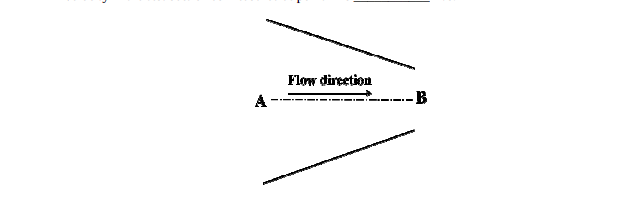
\includegraphics[width=0.5\columnwidth]{figs/Screenshot from 2025-08-16 11-34-10.png}
    \caption{Caption}
    \label{fig:placeholder}
\end{figure}



\item The rate of change of moment coefficient with respect to the angle of attack, $\frac{dC_m}{d\alpha}$, at half chord point of a thin airfoil, as per approximations from the thin airfoil theory is
\begin{enumerate}
\begin{multicols}{2}
    \item $\pi /4~\mathrm{radian}^{-1}$
    \item $\pi^2 / \mathrm{radian}^{-1}$
    \item $\pi~\mathrm{radian}^{-1}$
    \item $2\pi~\mathrm{radian}^{-1}$
\end{multicols}
\end{enumerate}
\hfill(GATE AE 2016)



\item An untwisted wing of elliptic planform and aspect ratio $6$ consists of thin symmetric airfoil sections. The coefficient of lift ($C_L$) at $10^{\degree}$ angle of attack assuming inviscid incompressible flow is
\begin{enumerate}
\begin{multicols}{2}
    \item $\pi^2/16$
    \item $\pi^2/12$
    \item $\pi^2/8$
    \item $\pi/2$
\end{multicols}
\end{enumerate}
\hfill(GATE AE 2016)



\item A gaseous mixture of air and fuel enters a constant area combustion chamber at a velocity of $100~\mathrm{m/s}$ and at a static temperature of $300~\mathrm{K}$. The heat release due to combustion is $1000~\mathrm{kJ/kg}$. The specific heat at constant pressure of the calorically perfect gas is $1000~\mathrm{J/kgK}$. The total temperature of air-fuel mixture after combustion is \dots K.
\hfill(GATE AE 2016)



\item Consider 1-D, steady, inviscid, compressible flow through a convergent nozzle. The total temperature and total pressure are $T_0$, $P_0$ respectively. The flow through the nozzle is choked with a mass flow rate of $\dot{m}_0$. If the total temperature is increased to $4T_0$, with total pressure remaining unchanged, then the mass flow rate through the nozzle
\begin{enumerate}
\begin{multicols}{2}
    \item remains unchanged.
    \item becomes half of $\dot{m}_0$.
    \item becomes twice of $\dot{m}_0$.
    \item becomes four times of $\dot{m}_0$.
\end{multicols}
\end{enumerate}
\hfill(GATE AE 2016)



\item Consider a second order linear ordinary differential equation 
$
\frac{d^2 y}{dx^2} - 4 \frac{dy}{dx} + 4y = 0,
$
with the boundary conditions $y(0) = 1$; $\left.\frac{dy}{dx}\right|_{x=0} = 1$. The value of $y$ at $x=1$ is
\begin{enumerate}
\begin{multicols}{2}
    \item $0$
    \item $1$
    \item $e$
    \item $e^2$
\end{multicols}
\end{enumerate}
\hfill(GATE AE 2016)



\item Consider the following system of linear equations:
$
\begin{aligned}
2x - y + z &= 1 
3x - 3y + 4z &= 6 
x - 2y + 3z &= 4
\end{aligned}
$
This system of linear equations has
\begin{enumerate}
\begin{multicols}{2}
    \item no solution.
    \item one solution.
    \item two solutions.
    \item three solutions.
\end{multicols}
\end{enumerate}
\hfill(GATE AE 2016)



\item A bar made of linear elastic isotropic material is fixed at one end and subjected to an axial force of $1~\mathrm{kN}$ at the other end. The cross-sectional area of the bar is $100~\mathrm{mm^2}$, length is $100~\mathrm{mm}$ and the Young's Modulus is $1 \times 10^5~\mathrm{N/mm^2}$. The strain energy stored in the bar is \dots Nmm.
\hfill(GATE AE 2016)



\item A cantilever beam-spring system is shown in the figure. The beam is made with a material of Young's modulus $1\times10^5~\mathrm{N/mm^2}$ and geometry such that its moment of inertia is $100~\mathrm{mm^4}$ and length $l = 100~\mathrm{mm}$. It is supported by a spring of stiffness $K = 30~\mathrm{N/mm}$ and subjected to a load of $P = 100~\mathrm{N}$ at the point 'B'. The deflection at the point 'B' due to the load $P$ is \dots mm.
\hfill(GATE AE 2016)

\begin{figure}[H]
    \centering
    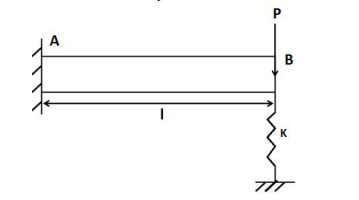
\includegraphics[width=0.5\columnwidth]{figs/Screenshot from 2025-08-16 11-44-28.png}
    \caption{Caption}
    \label{fig:placeholder}
\end{figure}



\item Determine the correctness or otherwise of the following statements, [a] and [r],
[a]: Ribs, used in airplane wings, increase the column buckling strength of the longitudinal stiffeners.
[r]: Ribs distribute concentrated loads into the structure and redistribute stresses around discontinuities.
\begin{enumerate}
    \item Both [a] and [r] are true and [r] is the correct reason for [a]
    \item Both [a] and [r] are true but [r] is not the correct reason for [a]
    \item Both [a] and [r] are false
    \item [a] is true but [r] is false
\end{enumerate}
\hfill(GATE AE 2016)



\item A channel section shown in the figure has uniform thickness. It is subjected to an anticlockwise torque of $62.5\times10^3~\mathrm{Nmm}$. The maximum possible thickness of the channel section, such that the shear stress induced in it does not exceed $100~\mathrm{N/mm^2}$, is \dots mm.
\hfill(GATE AE 2016)

\begin{figure}[H]
    \centering
    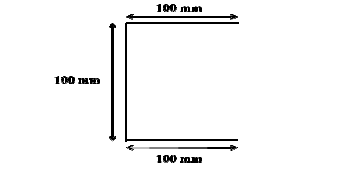
\includegraphics[width=0.5\columnwidth]{figs/Screenshot from 2025-08-16 11-47-37.png}
    \caption{Caption}
    \label{fig:placeholder}
\end{figure}



\item The governing differential equation of motion of a damped system is given by
$
m\frac{d^2 x}{dt^2} + c\frac{dx}{dt} + kx = 0
$
If $m = 1~\mathrm{kg},~c = 2~\mathrm{Ns/m}$ and $k = 2~\mathrm{N/m}$, then the frequency of the damped oscillation of this system is \dots rad/s.
\hfill(GATE AE 2016)



\item The two dimensional state of stress in a body is described by the Airy's stress function:
$
\phi = 5\frac{x^4}{12} + \frac{x^3y}{6} + \frac{x^2y^2}{2} + 7\frac{xy^3}{6} + E\frac{y^4}{12}
$
The Airy's stress function will satisfy the equilibrium and the compatibility requirements if and only if the value of the coefficient $E$ is \dots.
\hfill(GATE AE 2016)



\item The value of definite integral
$
\int_{0}^{\pi} (x \sin x)\, dx
$
is \dots.
\hfill(GATE AE 2016)



\item Use Newton-Raphson method to solve the equation: $x\,e^x = 1$. Begin with the initial guess $x_0 = 0.5$. The solution after one step is $x = $\dots.
\hfill(GATE AE 2016)



\item A wall of thickness $5~\mathrm{mm}$ is heated by a hot gas flowing along the wall. The gas is at a temperature of $3000~\mathrm{K}$, and the convective heat transfer coefficient is $160~\mathrm{W/m^2 K}$. The wall thermal conductivity is $40~\mathrm{W/mK}$. If the colder side of the wall is held at $500~\mathrm{K}$, the temperature of the side exposed to the hot gas is \dots K.
\hfill(GATE AE 2016)



\item A launch vehicle has a main rocket engine with two identical strap-on motors, all of which fire simultaneously during the operation. The main engine delivers a thrust of $6300~\mathrm{kN}$ with a specific impulse of $428~\mathrm{s}$. Each strap-on motor delivers a thrust of $12000~\mathrm{kN}$ with specific impulse of $292~\mathrm{s}$. The acceleration due to gravity is $9.81~\mathrm{m/s^2}$. The effective (combined) specific impulse of the vehicle is \dots s.
\hfill(GATE AE 2016)



\item A substance experiences an entropy change of $\Delta S > 0$ in a quasi-steady process. The rise in temperature (corresponding to the entropy change $\Delta S$) is highest for the following process:
\begin{enumerate}
\begin{multicols}{4}
    \item isenthalpic
    \item isobaric
    \item isochoric
    \item isothermal
\end{multicols}
\end{enumerate}
\hfill(GATE AE 2016)



\item In a particular rocket engine, helium propellant is heated to $6000~\mathrm{K}$ and $95\%$ of its total enthalpy is recovered as kinetic energy of the nozzle exhaust. Consider helium to be a calorically perfect gas with specific heat at constant pressure of $5200~\mathrm{J/kgK}$. The exhaust velocity for such a rocket for an optimum expansion is \dots m/s.
\hfill(GATE AE 2016)



\item An aircraft is flying level in the North direction at a velocity of $55~\mathrm{m/s}$ under cross wind from East to West of $5~\mathrm{m/s}$. For the given aircraft $C_{n\beta} = 0.012/\text{deg}$ and $C_{n\delta r} = -0.0072/\text{deg}$, where $\delta r$ is the rudder deflection and $\beta$ is the side slip angle. The rudder deflection exerted by pilot is \dots degrees.
\hfill(GATE AE 2016)



\item An aircraft weighing $10,000~\mathrm{N}$ is flying level at $100~\mathrm{m/s}$ and it is powered by a jet engine. The thrust required for level flight is $1000~\mathrm{N}$. The maximum possible thrust produced by the jet engine is $5000~\mathrm{N}$. The minimum time required to climb $1000~\mathrm{m}$, when flight speed is $100~\mathrm{m/s}$, is \dots s.
\hfill(GATE AE 2016)



\item The aircraft velocity (m/s) components in body axes are given as $[u, v, w] = [100, 10, 10]$. The air velocity (m/s), angle of attack (deg) and sideslip angle (deg) in that order are
\begin{enumerate}
\begin{multicols}{2}
    \item $[120, 0.1, 0.1]$
    \item $[100, 0.1, 0.1]$
    \item $[100.995, 0.1, 5.73]$
    \item $[100.995, 5.71, 5.68]$
\end{multicols}
\end{enumerate}
\hfill(GATE AE 2016)



\item The Dutch roll motion of the aircraft is described by following relationship

$
\myvec{\Delta \beta  \Delta r}
=
\myvec{-0.26 & -1  4.49 & -0.76}
\myvec{\Delta \beta  \Delta r}
$

The undamped natural frequency (rad/s) and damping ratio for the Dutch roll motion in that order are:
\begin{enumerate}
\begin{multicols}{4}
    \item $4.68,\ 1.02$
    \item $4.49,\ 1.02$
    \item $2.165,\ 0.235$
    \item $2.165,\ 1.02$
\end{multicols}
\end{enumerate}
\hfill(GATE AE 2016)



\item A glider weighing $3300~\mathrm{N}$ is flying at $1000~\mathrm{m}$ above sea level. The wing area is $14.1~\mathrm{m^2}$ and the air density is $1.23~\mathrm{kg/m^3}$. Under zero wind conditions, the velocity for maximum range is \dots m/s.

\begin{center}
\begin{tabular}{|c|c|c|}
\hline
\textbf{Mineral} & \textbf{Entropy $S^{1,823}$ (kJ K$^{-1}$)} & \textbf{Volume $V^{1,823}$ (J bar$^{-1}$)} \\
\hline
Grossular   & 0.255 & 12.535 \\
\hline
Quartz      & 0.042 & 2.269 \\
\hline
Anorthite   & 0.200 & 10.079 \\
\hline
Wollastonite & 0.082 & 3.993 \\
\hline
\end{tabular}    
\end{center}



\hfill(GATE AE 2016)



\item A rocket, with a total lift-off mass of $10,000~\mathrm{kg}$, moves vertically upward from rest under a constant gravitational acceleration of $9.81~\mathrm{m/s^2}$. The propellant mass of $8400~\mathrm{kg}$ burns at a constant rate of $1200~\mathrm{kg/s}$. If the specific impulse of the rocket engine is $240~\mathrm{s}$, neglecting drag, the burnout velocity in m/s is
\begin{enumerate}
\begin{multicols}{4}
    \item $3933.7$
    \item $4314.6$
    \item $4245.9$
    \item $4383.3$
\end{multicols}
\end{enumerate}
\hfill(GATE AE 2016)



\item A satellite is injected at an altitude of $350~\mathrm{km}$ above the Earth's surface, with a velocity of $8.0~\mathrm{km/s}$ parallel to the local horizon. (Earth radius $= 6378~\mathrm{km}$, $\mu_E$ (GM = Gravitational constant $\times$Earth mass) $= 3.986 \times 10^{14}~\mathrm{m^3~s^{-2}}$. The satellite
\begin{enumerate}
\begin{multicols}{2}
    \item forms a circular orbit.
    \item forms an elliptic orbit.
    \item escapes from Earth's gravitational field.
    \item falls back to earth.
\end{multicols}
\end{enumerate}
\hfill(GATE AE 2016)


 \newpage

 \setlength{\fboxsep}{6pt} % padding inside the box

\begin{center}
\fbox{%
  \begin{minipage}{0.96\textwidth}
    \underline{\textbf{Useful data}}\\[6pt]

    \begin{tabular}{l l}
      Avogadro's Number & : $6.023\times10^{23}\ \mathrm{mol^{-1}}$\\[4pt]
      Boltzmann's constant & : $1.38\times10^{-23}\ \mathrm{J\ K^{-1}}$\\[4pt]
      Electron Charge & : $1.6\times10^{-19}\ \mathrm{C}$\\[4pt]
      Gas Constant & : $8.314\ \mathrm{J\ mol^{-1}\ K^{-1}}$\\[4pt]
      Electron rest mass & : $9.1\times10^{-31}\ \mathrm{kg}$\\[4pt]
      Permittivity of vacuum ($\varepsilon_0$) & : $8.854\times10^{-12}\ \mathrm{F\ m^{-1}}$\\[4pt]
      Planck's constant ($h$) & : $6.62\times10^{-34}\ \mathrm{J\ s^{-1}}$\\[4pt]
      Bohr Magneton ($\mu_B$) & : $9.27\times10^{-24}\ \mathrm{A\ m^{2}}$\\
    \end{tabular}

    \vspace{8pt}

    $1\ \mathrm{eV} = 1.6\times10^{-19}\ \mathrm{J}$\\[2pt]
    $1\ \mathrm{cal} = 4.2\ \mathrm{J}$

    \vspace{10pt}

    \textbf{Atomic weight (in kg mol$^{-1}$) of:}\\[6pt]
    \begin{tabular}{l l}
      Hydrogen & 0.001\\
      Carbon   & 0.012\\
      Nitrogen & 0.014
    \end{tabular}

  \end{minipage}%
}%
\end{center}

 
\end{enumerate}
\end{document}